\PassOptionsToPackage{table,xcdraw,dvipsnames}{xcolor}
\documentclass[aspectratio=169,10pt]{beamer}

\usetheme{Madrid}
\usecolortheme{default}

\definecolor{sfaxblue}{RGB}{0,51,102}
\definecolor{sfaxgold}{RGB}{204,153,0}
\definecolor{softblue}{RGB}{233,242,248}
\definecolor{softgray}{RGB}{245,245,245}
\definecolor{accentgreen}{RGB}{35,130,75}
\definecolor{accentred}{RGB}{170,45,45}
\definecolor{accentorange}{RGB}{200,110,20}

\setbeamercolor{palette primary}{bg=sfaxblue,fg=white}
\setbeamercolor{palette secondary}{bg=sfaxblue!85,fg=white}
\setbeamercolor{palette tertiary}{bg=sfaxblue!70,fg=white}
\setbeamercolor{palette quaternary}{bg=sfaxgold,fg=sfaxblue}
\setbeamercolor{structure}{fg=sfaxblue}
\setbeamercolor{frametitle}{bg=sfaxblue,fg=white}
\setbeamercolor{block title}{bg=sfaxblue,fg=white}
\setbeamercolor{block body}{bg=softblue,fg=black}
\setbeamercolor{item}{fg=sfaxblue}

\usepackage[utf8]{inputenc}
\usepackage[T1]{fontenc}
\usepackage{lmodern}
\usepackage{microtype}
\usepackage{booktabs}
\usepackage{tabularx}
\usepackage{array}
\usepackage{tikz}
\usetikzlibrary{positioning,arrows.meta,shapes.geometric,fit,calc}
\usepackage{fontawesome5}

\setbeamertemplate{navigation symbols}{}
\setbeamertemplate{itemize item}{\color{sfaxgold}\textbullet}
\setbeamertemplate{itemize subitem}{\color{sfaxblue}\scriptsize\faAngleRight}
\setbeamertemplate{footline}{
  \leavevmode
  \hbox{
    \begin{beamercolorbox}[wd=.30\paperwidth,ht=2.5ex,dp=1.5ex,center]{palette secondary}
      Ahmedou Yahye Kheyri
    \end{beamercolorbox}
    \begin{beamercolorbox}[wd=.45\paperwidth,ht=2.5ex,dp=1.5ex,center]{palette tertiary}
      State of the Art and Methodology
    \end{beamercolorbox}
    \begin{beamercolorbox}[wd=.25\paperwidth,ht=2.5ex,dp=1.5ex,right]{palette quaternary}
      \insertframenumber/\inserttotalframenumber\hspace*{2ex}
    \end{beamercolorbox}
  }
}

\title[\textsc{SOTA} and Methodology]{\textbf{From IaC Security Smell Detection}\\\textbf{to Agentic Remediation}}
\subtitle{State of the Art and Methodology for Reliable IaC Security Fixing}
\author{Ahmedou Yahye Kheyri \\ \small Supervised by Prof.\ Hala Bezine}
\institute{Faculty of Sciences of Sfax \\ Master MRSI \\ 2025--2026}
\date{May 2026}

\begin{document}

{
\setbeamertemplate{footline}{}
\begin{frame}[plain]
\begin{tikzpicture}[remember picture,overlay]
  \fill[sfaxblue] ([yshift=-0.07\paperheight]current page.north west)
    rectangle (current page.north east);
  \fill[sfaxgold] ([yshift=-0.02\paperheight]current page.north west)
    rectangle ([yshift=-0.035\paperheight]current page.north east);
  \fill[sfaxgold] ([yshift=0.05\paperheight]current page.south west)
    rectangle ([yshift=0.065\paperheight]current page.south east);
\end{tikzpicture}

\vspace*{1.5cm}
{\color{sfaxblue}\LARGE\textbf{From IaC Security Smell Detection}}\\[0.15cm]
{\color{sfaxblue}\LARGE\textbf{to Agentic Remediation}}\\[0.45cm]
{\color{sfaxblue}\large State of the Art and Research Methodology}\\[0.55cm]
{\color{sfaxgold}\rule{0.78\linewidth}{1.2pt}}\\[0.55cm]
{\color{black!80}\normalsize Detecting, analyzing, and reliably remediating Infrastructure-as-Code security misconfigurations}\\[0.7cm]

\begin{tabular}{@{}ll@{}}
  {\color{sfaxgold}\faUserGraduate} & {\color{sfaxblue}\textbf{Ahmedou Yahye Kheyri}} \\
  {\color{sfaxgold}\faChalkboardTeacher} & {\color{black!80}Supervised by Prof.\ Hala Bezine} \\
  {\color{sfaxgold}\faUniversity} & {\color{black!80}Faculty of Sciences of Sfax --- Master MRSI} \\
  {\color{sfaxgold}\faCalendar} & {\color{black!80}May 2026}
\end{tabular}

\vfill
\end{frame}
}

\begin{frame}{Research Question}
\begin{block}{State-of-the-art question}
What existing methods detect, analyze, and remediate Infrastructure-as-Code security misconfigurations, and what are their limits?
\end{block}
\begin{alertblock}{Scientific position}
Existing IaC security tools detect misconfigurations, and LLM/RAG systems can suggest fixes, but reliable automatic remediation requires a validation loop with external analyzers.
\end{alertblock}
\end{frame}

\begin{frame}{1. IaC Security Problems}
\begin{columns}[T]
\begin{column}{0.5\textwidth}
\begin{block}{Why IaC matters}
\small
IaC scripts such as Terraform, Kubernetes YAML, Ansible, Dockerfiles, and CloudFormation configure real infrastructure directly.
\end{block}
\begin{block}{Typical security risks}
\small
\begin{itemize}
  \item hardcoded secrets
  \item public access and weak network exposure
  \item excessive privileges
  \item weak encryption settings
  \item privileged containers
  \item missing integrity checks
\end{itemize}
\end{block}
\end{column}
\begin{column}{0.47\textwidth}
\begin{block}{Core challenge}
\small
Misconfigurations are dangerous, frequent, and often context-dependent.
\end{block}
\begin{block}{Implication for research}
\small
The problem is not only detecting insecure IaC, but also producing trustworthy remediation that works on the real artifact.
\end{block}
\end{column}
\end{columns}
\end{frame}

\begin{frame}{2. Security Smells and Taxonomies}
\begin{tabularx}{\linewidth}{>{\raggedright\arraybackslash}p{2.8cm}X}
\toprule
\textbf{Period} & \textbf{Main idea} \\
\midrule
Early works & Security smells studied in Puppet, Ansible, and Chef scripts. \\
Seven Sins era & Small taxonomies of recurring IaC security smells became established. \\
GLITCH era & Polyglot detection across multiple IaC technologies. \\
Recent updates & Larger smell taxonomies with broad tool coverage, reaching 62 categories across seven IaC tools. \\
\bottomrule
\end{tabularx}
\vspace{0.4cm}
\begin{alertblock}{Main observation}
Detection taxonomies are becoming mature, but remediation remains much less explored.
\end{alertblock}
\end{frame}

\begin{frame}{3. Static Analysis Tools for IaC}
\begin{columns}[T]
\begin{column}{0.48\textwidth}
\begin{block}{Representative tools}
\small
\begin{itemize}
  \item Checkov
  \item Terrascan
  \item tfsec / Trivy
  \item KICS
  \item GLITCH
  \item policy-as-code tools
\end{itemize}
\end{block}
\end{column}
\begin{column}{0.48\textwidth}
\begin{block}{Limits}
\small
\begin{itemize}
  \item strong at detecting known rule violations
  \item often limited to alerts or generic advice
  \item weak contextual remediation support
  \item little verification of automated fixes
\end{itemize}
\end{block}
\end{column}
\end{columns}
\vspace{0.35cm}
\begin{alertblock}{Gap}
Static analyzers are effective for detection, but remediation usually remains manual, rule-based, or weakly contextualized.
\end{alertblock}
\end{frame}

\begin{frame}{4. LLMs for Code Security and IaC}
\begin{block}{What LLMs add}
\small
LLMs can generate code, explain vulnerabilities, and propose patches for insecure artifacts.
\end{block}
\begin{itemize}
  \item useful for patch suggestion and security explanation
  \item able to leverage natural-language and code context
  \item recent IaC-focused work such as GenSIaC moves toward security-aware generation
  \item but generated fixes may hallucinate, fail validation, or introduce new problems
\end{itemize}
\vspace{0.35cm}
\begin{alertblock}{Limit}
LLM-based remediation is promising, but textually plausible fixes are not necessarily operationally correct or secure.
\end{alertblock}
\end{frame}

\begin{frame}{5. RAG for Security and Code Assistance}
\begin{block}{Basic idea}
\small
RAG grounds generation by retrieving external knowledge instead of relying only on the model's internal parameters.
\end{block}
\begin{itemize}
  \item secure IaC examples
  \item scanner rule documentation
  \item CWE descriptions
  \item before/after security fixes
  \item cloud security guidelines and best practices
\end{itemize}
\vspace{0.35cm}
\begin{alertblock}{Limit}
Basic RAG improves grounding, but retrieval can still be noisy, incomplete, or irrelevant, which means the final patch can still fail.
\end{alertblock}
\end{frame}

\begin{frame}{6. Advanced RAG: Self-RAG and CRAG}
\begin{block}{Why advanced RAG matters}
\small
More recent systems do not trust one retrieval pass and one generation pass.
\end{block}
\begin{itemize}
  \item Self-RAG adds self-reflection and critique
  \item CRAG adds retrieval evaluation and corrective retrieval behavior
  \item both move from passive retrieval to controlled, quality-aware generation
\end{itemize}
\vspace{0.35cm}
\begin{alertblock}{Relevance to this work}
These ideas motivate a remediation loop in which retrieved knowledge, generation quality, and correction are treated as uncertain.
\end{alertblock}
\end{frame}

\begin{frame}{7. Tool-Using and Agentic LLMs}
\begin{columns}[T]
\begin{column}{0.48\textwidth}
\begin{block}{Tool use}
\small
Toolformer and later agentic systems show that language models can call external tools instead of acting as pure text generators.
\end{block}
\end{column}
\begin{column}{0.48\textwidth}
\begin{block}{Relevant tools for IaC}
\small
\begin{itemize}
  \item Checkov
  \item KICS
  \item Terrascan
  \item Terraform validators
  \item YAML and manifest checkers
  \item policy engines
\end{itemize}
\end{block}
\end{column}
\end{columns}
\vspace{0.35cm}
\begin{alertblock}{Key idea}
The language model can act as an agent that interacts with analyzers to verify and improve candidate fixes.
\end{alertblock}
\end{frame}

\begin{frame}{State-of-the-Art Logic}
\centering
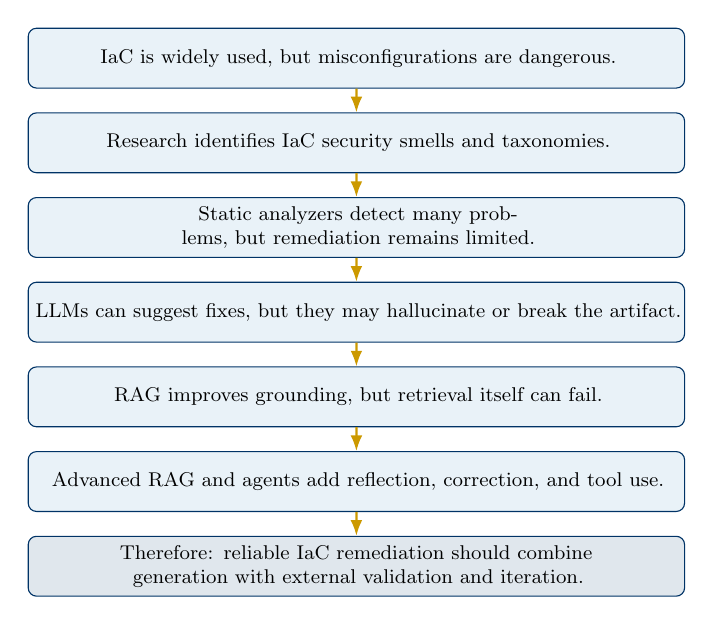
\begin{tikzpicture}[
  scale=0.8,
  transform shape,
  node distance=0.38cm,
  logic/.style={draw=sfaxblue, rounded corners=3pt, fill=softblue, text width=0.84\linewidth, align=center, minimum height=0.95cm, font=\small},
  arr/.style={-{Latex[length=2mm]}, thick, sfaxgold}
]
\node[logic] (a) {IaC is widely used, but misconfigurations are dangerous.};
\node[logic, below=of a] (b) {Research identifies IaC security smells and taxonomies.};
\node[logic, below=of b] (c) {Static analyzers detect many problems, but remediation remains limited.};
\node[logic, below=of c] (d) {LLMs can suggest fixes, but they may hallucinate or break the artifact.};
\node[logic, below=of d] (e) {RAG improves grounding, but retrieval itself can fail.};
\node[logic, below=of e] (f) {Advanced RAG and agents add reflection, correction, and tool use.};
\node[logic, below=of f, fill=sfaxblue!12] (g) {Therefore: reliable IaC remediation should combine generation with external validation and iteration.};
\draw[arr] (a) -- (b);
\draw[arr] (b) -- (c);
\draw[arr] (c) -- (d);
\draw[arr] (d) -- (e);
\draw[arr] (e) -- (f);
\draw[arr] (f) -- (g);
\end{tikzpicture}
\end{frame}

\begin{frame}{Main Research Gap}
\begin{block}{Gap statement}
Existing IaC security research has made strong progress in smell detection,
taxonomy construction, and static analysis. However, less attention has been
given to reliable automatic remediation.
\end{block}
\begin{itemize}
  \item static analyzers identify misconfigurations but usually provide limited contextual fixes
  \item LLM-based approaches can generate patches but may hallucinate or introduce new errors
  \item reliable remediation therefore requires retrieval, generation, validation, and iterative improvement
\end{itemize}
\end{frame}

\begin{frame}{Proposed Framework}
\centering
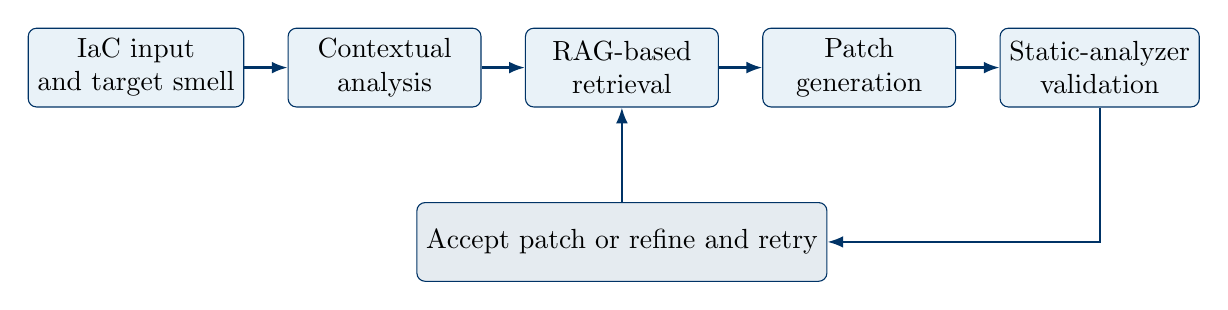
\begin{tikzpicture}[
  node distance=0.9cm and 0.55cm,
  box/.style={draw=sfaxblue, rounded corners=3pt, fill=softblue, minimum width=2.45cm, minimum height=1.0cm, align=center},
  widebox/.style={draw=sfaxblue, rounded corners=3pt, fill=sfaxblue!10, minimum width=3.1cm, minimum height=1.0cm, align=center},
  arrow/.style={-{Latex[length=2mm]}, thick, sfaxblue}
]
\node[box] (a) {IaC input\\and target smell};
\node[box, right=of a] (b) {Contextual\\analysis};
\node[box, right=of b] (c) {RAG-based\\retrieval};
\node[box, right=of c] (d) {Patch\\generation};
\node[box, right=of d] (e) {Static-analyzer\\validation};
\node[widebox, below=1.2cm of c] (f) {Accept patch or refine and retry};
\draw[arrow] (a) -- (b);
\draw[arrow] (b) -- (c);
\draw[arrow] (c) -- (d);
\draw[arrow] (d) -- (e);
\draw[arrow] (e.south) |- (f.east);
\draw[arrow] (f.north) -| (c.south);
\end{tikzpicture}
\vspace{0.4cm}
\begin{itemize}
  \item candidate patches are accepted only after external validation
  \item the remediation loop combines retrieval, generation, testing, and refinement
\end{itemize}
\end{frame}

\begin{frame}{Evaluation Logic}
\begin{tabularx}{\linewidth}{>{\raggedright\arraybackslash}p{3cm}X}
\toprule
\textbf{Metric family} & \textbf{Question answered} \\
\midrule
Patch validity & Is the produced patch syntactically and operationally acceptable? \\
Smell elimination & Does the targeted issue disappear after remediation? \\
No-new-issues & Does the fix avoid introducing additional scanner findings? \\
Cross-validator agreement & Do Checkov and KICS support the same acceptance decision? \\
Qualitative failure analysis & Why do failures happen: retrieval mismatch, weak patch, validator conflict, or incomplete context? \\
\bottomrule
\end{tabularx}
\end{frame}

\begin{frame}{Experimental Direction}
\begin{block}{Evaluation objective}
The framework must be assessed empirically on real IaC artifacts and validated with independent analyzers.
\end{block}
\begin{itemize}
  \item freeze the training and evaluation splits
  \item prepare Kaggle experiments for QLoRA fine-tuning
  \item evaluate selected system configurations
  \item collect quantitative results and qualitative remediation examples
  \item compare patch validity, smell elimination, and no-new-issues behavior
\end{itemize}
\end{frame}

\begin{frame}{Expected Outcomes}
\begin{columns}[T]
\begin{column}{0.48\textwidth}
\begin{block}{Scientific contribution}
\small
\begin{itemize}
  \item focused state of the art
  \item explicit research gap
  \item methodology for validated remediation
  \item clear positioning in the literature
\end{itemize}
\end{block}
\end{column}
\begin{column}{0.48\textwidth}
\begin{block}{Empirical contribution}
\small
\begin{itemize}
  \item Kaggle training logs
  \item validated test results
  \item comparison tables
  \item journal-ready figures and discussion
\end{itemize}
\end{block}
\end{column}
\end{columns}
\vspace{0.4cm}
\begin{alertblock}{Bottom line}
The research positioning is clear, but the strength of the final contribution
depends on rigorous experimental validation.
\end{alertblock}
\end{frame}

\begin{frame}
\centering
\vspace{1.5cm}
{\Huge Thank you}\\[0.6cm]
{\large Questions and discussion}
\end{frame}

\end{document}
